\chapter{相关技术介绍}\label{ux7b2cux4e8cux7ae0-ux76f8ux5173ux6280ux672fux4ecbux7ecd}

本章介绍本作品涉及的基础技术，包括语音合成、语音克隆、语音表示、语音分词器、说话人识别、对抗攻击与主动防护、听觉感知约束和音频质量评价。整体上，本章为第三章系统设计与实现提供技术背景，重点回答三个问题：第一，语音克隆系统为什么能够从公开音频中学习目标声音；第二，机器模型通常从语音中提取哪些信息；第三，为什么可以通过发布前保护扰动降低未授权语音克隆的风险。

\section{语音合成与语音克隆技术}\label{ux8bedux97f3ux5408ux6210ux4e0eux8bedux97f3ux514bux9686ux6280ux672f}

语音合成技术的发展是声音资产安全问题产生的直接技术背景。早期语音合成主要解决``让机器把文字读出来''的问题，而现代语音合成已经逐渐发展为可以生成自然语音、控制说话人身份、迁移语音风格甚至复刻目标说话人声音特征的生成式技术。随着零样本语音克隆、少样本微调和基于大语言模型的语音合成不断发展，公开语音样本不再只是普通音频内容，也可能成为语音克隆系统提取声音身份信息的参考材料。

\subsection{传统与深度神经网络语音合成}\label{ux4f20ux7edfux4e0eux6df1ux5ea6ux795eux7ecfux7f51ux7edcux8bedux97f3ux5408ux6210}

传统语音合成通常分为拼接式、参数式及统计参数语音合成三类。拼接式方法依赖大规模语音片段库，通过选取并拼接合适单元生成语音，在固定场景下自然度较高，但对语料覆盖、录制质量和拼接平滑性要求严苛，系统灵活性有限。参数式和统计参数式方法则将语音生成转化为声学参数预测，从文本提取语言学特征后预测基频、频谱等参数并通过声码器还原波形，虽较拼接式更为灵活，但生成的语音往往存在机械感，音色细节、韵律自然度及情感表现力不足。

传统语音合成对声音资产安全的威胁相对有限，因其通常依赖大量目标语音、复杂人工处理和较高工程成本。而深度神经网络语音合成的出现，显著增强了模型对语音内容、说话人身份和声学条件的学习能力，使语音克隆风险逐渐从专业系统层面扩散为普通用户也可能面对的现实威胁。

深度神经网络语音合成（Neural
Text-to-Speech）使用神经网络学习文本到声学表示、声学表示到波形之间的映射关系。Tacotron
2
将输入字符序列转换为梅尔频谱，再由神经声码器生成最终波形，推动了端到端神经语音合成的发展\textsuperscript{{[}1{]}}。FastSpeech
采用非自回归结构生成声学特征，提高了合成速度和稳定性\textsuperscript{{[}2{]}}。FastSpeech
2
进一步引入时长、基频和能量等变化信息，使模型能够更直接地控制语音节奏、音高和能量变化\textsuperscript{{[}3{]}}。VITS
则通过条件变分自编码器、标准化流和对抗训练实现端到端文本到语音合成，在自然度和工程简化方面具有代表性\textsuperscript{{[}4{]}}。

从防护角度看，深度神经网络语音合成的重要变化在于：模型不再只依赖人工规则，而是能够从大量语音数据中学习复杂的声音规律。语音内容、音素结构、说话人身份、音色、韵律、风格和声学环境都可能以不同形式被编码到模型中。也就是说，公开语音样本不仅包含人耳听到的内容，还包含机器可学习的声音身份信息。

因此，V-Guard
在设计防护目标时，不能只把语音看作普通波形文件，而应将其视为同时承载语义信息和声音身份信息的机器输入。语义信息主要进入语义表示链路，声音身份信息主要进入声音身份特征链路。后续主动防护设计正是围绕这两类机器依赖展开。如图
2-1 展示了双链路相关的特征提取。


\begin{figure}[htbp]
  \centering
  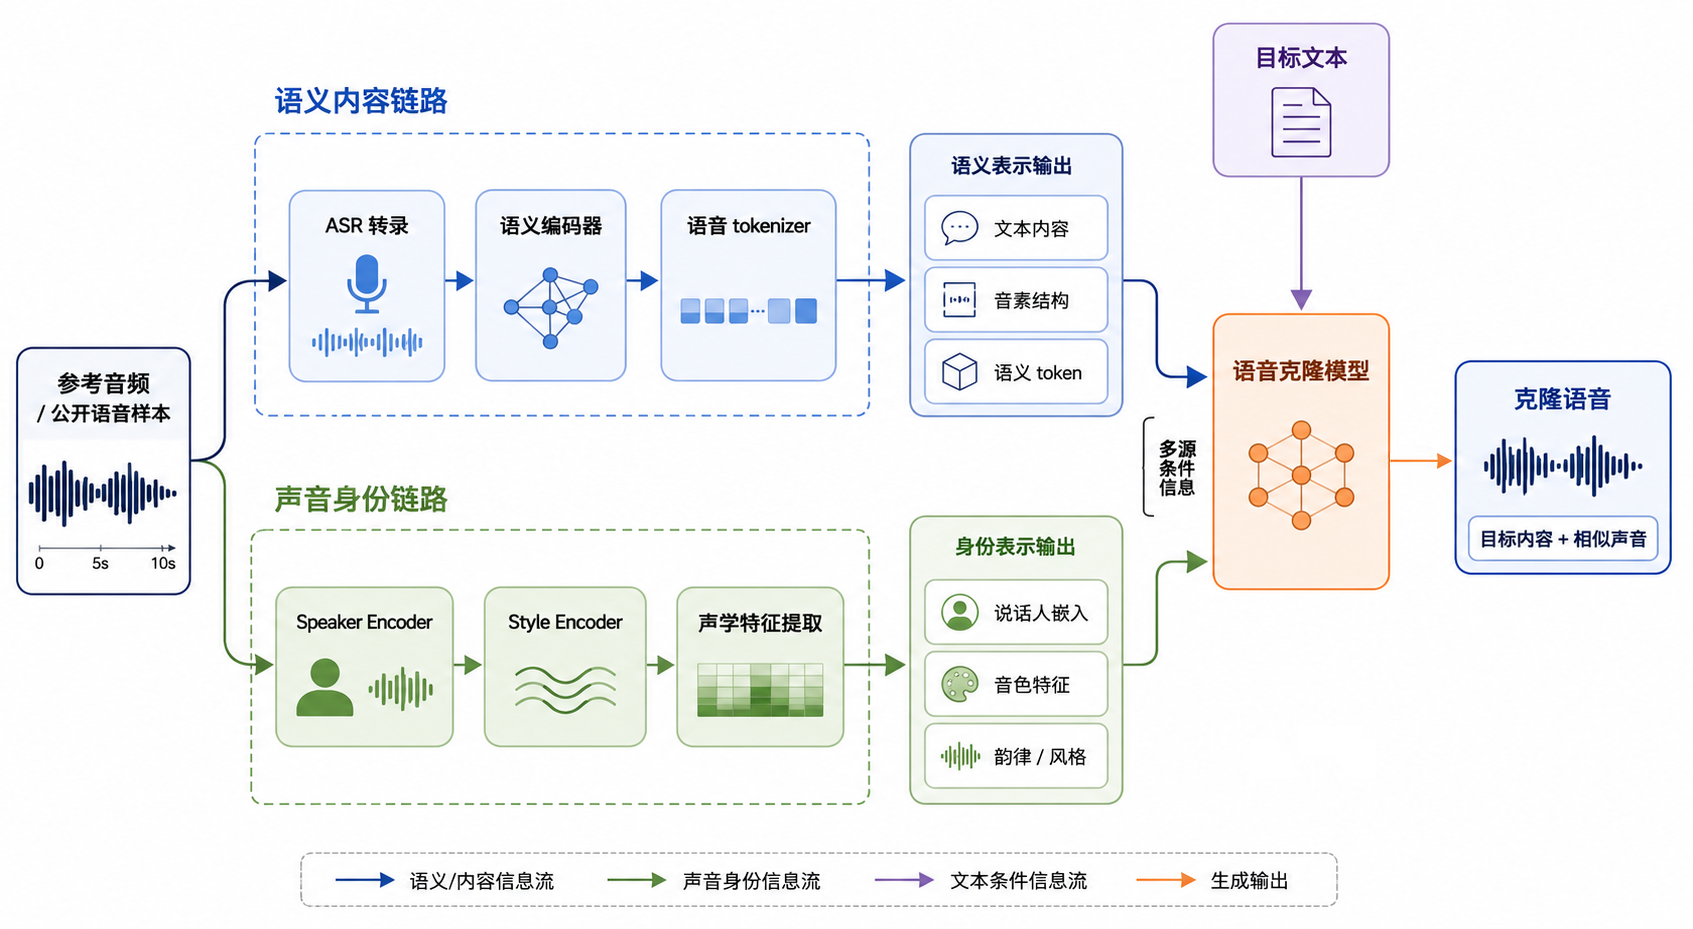
\includegraphics[width=\textwidth,height=0.72\textheight,keepaspectratio]{figures/image4.png}
  \caption{语音克隆对参考音频的信息提取链路示意图}
  \label{fig:2-1}
\end{figure}

\subsection{现代语音克隆与大模型语音合成}\label{ux73b0ux4ee3ux8bedux97f3ux514bux9686ux4e0eux5927ux6a21ux578bux8bedux97f3ux5408ux6210}

现代语音克隆技术进一步降低了目标声音复刻门槛。零样本语音克隆通常只需要一段短参考语音和一段目标文本，就可能生成具有相似声音特征的语音。少样本或微调式语音克隆则通过收集多条目标说话人语音，对已有模型进行适配或微调，从而更稳定地学习目标说话人的声音身份信息。YourTTS
等工作体现了零样本多说话人语音合成和语音转换的发展方向\textsuperscript{{[}11{]}}。

基于大语言模型的语音合成（LLM-based TTS，Large Language Model-based
Text-to-Speech）进一步改变了语音建模方式。VALL-E
将文本到语音合成建模为基于神经音频编码离散码的条件语言建模任务，说明离散语音编码可以成为零样本语音合成的重要中间表示\textsuperscript{{[}5{]}}。CosyVoice
使用监督语义
token，并结合大语言模型式生成结构提升多语言零样本语音合成能力\textsuperscript{{[}6{]}}。这类方法表明，语音合成系统可能不再只依赖传统连续声学特征，也可能通过语音分词器将语音转换为离散语音
token，再交由后续语言模型进行建模{[}13-18{]}。

从安全角度看，现代语音克隆攻击可能出现在多个阶段。攻击者可以直接在推理阶段输入目标文本和参考语音，生成目标说话人的克隆语音；也可以先利用自动语音识别（ASR，Automatic
Speech
Recognition）为公开语音生成文本标注，再构造文本---音频训练对；还可以收集多条受害者语音后进行少样本微调。因此，对公开语音的防护不能只面向最终合成结果，还应当面向参考音频被编码、标注、微调和推理利用的整个前端信息提取过程。

V-Guard
的发布前主动防护正是针对这一特点：只要攻击者使用的是公开发布后的受保护音频，保护扰动就可能在训练数据构造、微调学习和推理参考条件中持续影响机器模型对原始声音资产的提取。

\section{语音表示与语音分词器}\label{ux8bedux97f3ux8868ux793aux4e0eux8bedux97f3ux5206ux8bcdux5668}

语音模型无法直接使用``人耳听到的声音''进行推理，而是需要先将原始波形转换为机器可处理的表示。不同模型的表示形式不同，有的依赖梅尔频谱、梅尔频率倒谱系数等显式声学特征，有的直接从波形中学习连续隐藏表示，还有的进一步将连续表示量化为离散语音
token{[}28-41{]}。理解这些表示形式，有助于解释为什么保护扰动可以在不明显影响人耳听感的情况下影响机器识别和语音克隆。

\subsection{声学特征、连续表示与语音分词器}\label{ux58f0ux5b66ux7279ux5f81ux8fdeux7eedux8868ux793aux4e0eux8bedux97f3ux5206ux8bcdux5668}

传统语音处理系统通常会先从原始波形中提取声学特征。常见声学特征包括短时傅里叶变换（STFT，Short-Time
Fourier Transform）、梅尔频谱图（Mel
Spectrogram）、对数梅尔频谱图（Log-Mel
Spectrogram）和梅尔频率倒谱系数（MFCC，Mel-Frequency Cepstral
Coefficients）。这些特征从时间、频率和能量分布角度描述语音信号，使模型能够分析发音结构、频带变化和声音强度。

在深度学习语音模型中，声学特征并不一定以人工设计形式出现。wav2vec 2.0
直接从语音中学习潜在表示，并在潜在空间中进行掩码和对比学习\textsuperscript{{[}37{]}}。HuBERT
通过掩码预测隐藏单元的方式进行自监督语音表示学习\textsuperscript{{[}38{]}}。WavLM
面向更完整的语音处理任务学习通用表示，其研究背景明确指出语音信号包含说话内容、说话人身份、副语言信息等多方面内容\textsuperscript{{[}39{]}}。Whisper
则通过大规模弱监督语音识别训练获得较强的跨语种和鲁棒识别能力\textsuperscript{{[}40{]}}。

上述模型说明，现代语音系统中的连续表示并不是简单的波形复制，而是机器对语音内容、发音结构、说话人身份、声学环境等信息的高维编码。V-Guard
中的语义表示和声音身份表示，都可以理解为这种连续表示在不同防护目标下的功能划分。语义表示更关注``说了什么''，声音身份表示更关注``是谁在说、怎么说''。

语音分词器（Speech Tokenizer）是连接连续语音信号与离散语音 token
的关键模块。它通常接收原始波形或声学特征，先通过编码器得到连续隐藏表示，再通过量化器将连续表示映射为离散索引序列。与文本分词器将文本拆分为字符、子词或词元不同，语音分词器处理的是连续音频信号，其输出可以作为语音大模型、神经音频编解码器或基于
token 的语音生成系统的输入。

离散语音 token（Discrete Speech Token）可以分为不同层次。一类 token
更偏向语义内容，可能承载语音内容、音素结构和发音时序等信息；另一类 token
更偏向声学细节，可能承载音色、韵律、风格、环境和重建波形所需的信息。SpeechTokenizer
明确提出统一语音分词器结构，并区分语义 token 和声学
token，同时采用编码器---解码器结构和残差向量量化（RVQ，Residual Vector
Quantization）\textsuperscript{{[}31{]}}。

需要强调的是，本文并不把语音分词器写成所有语音克隆系统的共同必经模块。传统自动语音识别、说话人验证、连续表示型语音克隆和部分微调式语音合成系统可能直接使用连续隐藏表示，而不显式产生离散语音
token。因此，V-Guard 在后续方法中采用``连续表示主干 + 可选离散语音 token
分支''的理解方式：对于连续表示型系统，保护扰动主要影响连续语义表示和声音身份表示；对于基于语音分词器的新型系统，连续表示偏移还可能进一步影响离散
token 的选择。

\subsection{语音编码器表征机理与量化机制}\label{ux8bedux97f3ux7f16ux7801ux5668ux8868ux5f81ux673aux7406ux4e0eux91cfux5316ux673aux5236}

为了确保提取的表示能精准表征``语音身份''、``语义''或者``噪声''等抽象音频特征，系统会采用代理编码器在底层数学拓扑上建立一套严密的特征解耦机制，用于提取语音表示的某一特征，如音色、说话者身份、语义等等。

在本文的背景下，我们主要关注有关语音身份和语义方面的代理编码器，以语音身份代理编码器为例，它们实现精准特征提取的核心机理如下：


\begin{figure}[htbp]
  \centering
  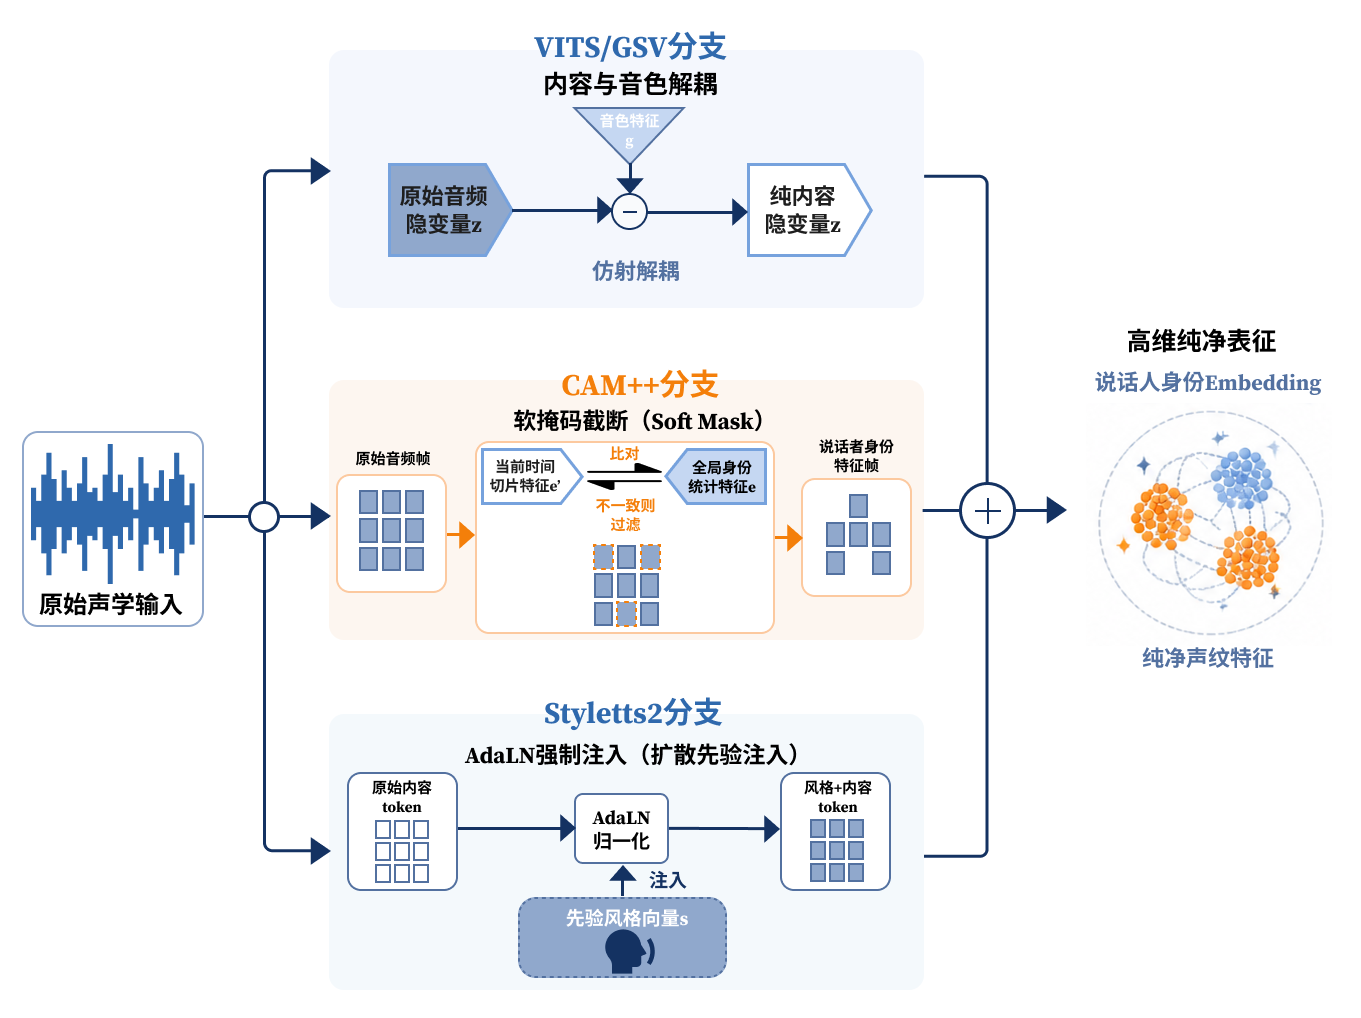
\includegraphics[width=\textwidth,height=0.72\textheight,keepaspectratio]{figures/image5.png}
  \caption{代理编码器}
  \label{fig:2-2}
\end{figure}

\begin{enumerate}
\def\labelenumi{(\arabic{enumi})}
\item
  TTS 后验编码器（VITS/GSV）：基于可逆流的音色物理剥离\\
  在 TTS 后验编码器中，其核心理念是通过标准化流（Normalizing
  Flows）实现音色的物理级剥离。网络强制将隐变量解构为纯净的内容表达，而音色特征被提取为全局条件向量
  \(g\)。具体而言，这一解耦过程通过仿射耦合映射来实现，其核心公式为：
\end{enumerate}

\[z_{p}^{(i)} = \left( z^{(i)} - \mu(z^{( < i)},g) \right) \odot exp\left( - \sigma(z^{( < i)},g) \right)\]

网络利用音色向量 \(g\)
生成平移（\(\mu\)）和缩放（\(\sigma\)）参数，精准抵消原始隐变量内部的音色分量。这种设计从物理计算层面确保了音色与内容的绝对正交解耦。

\begin{enumerate}
\def\labelenumi{(\arabic{enumi})}
\setcounter{enumi}{1}
\item
  说话人验证网络（CAM++）：基于上下文掩码的高维聚类\\
  CAM++
  这类说话人验证网络，其终极任务是判断两句话是不是同一个人说的。但神经网络不能直接对比两段长短不一、内容不同的波形。为了完成对比，网络必须在其结构的深层（也就是输出最终的
  yes/no
  之前），将输入的超长音频压缩成一个固定维度的向量。这个特征向量剥离了内容、情感等等无关因素，只留下了代表说话人音色特征的声纹嵌入（Speaker
  Embedding）。这一过程通过密集连接与显式的软掩码机制，动态阻断非目标噪声或无关发音帧的干扰，从而促使说话人身份在隐空间中形成极其致密的聚类球体，其上下文感知门控截断机制的核心公式为：\\
  \[{\widetilde{X}}_{t} = M_{k} \odot X_{t}\quad\text{其中}\quad M_{k} = \sigma\left( W_{2} \cdot \text{ReLU}\left( W_{1}(e_{g} + e_{k}^{s}) + b_{1} \right) + b_{2} \right)\]
\end{enumerate}

公式中的 \(e_{g}\)
代表整段音频的``全局身份统计量''（即该说话人的总体声纹基准），而
\(e_{k}^{s}\)
代表当前这一微小时间切片内的``局部特征''。在实际运算中，掩码 \(M_{k}\)
会实时对比局部切片特征（\(e_{k}^{s}\)）与全局身份统计量（\(e_{g}\)）。最外层的
\(\sigma\)
函数会过滤掉无关的噪声。一旦检测到当前帧偏离了全局的声纹流形，网络便会输出趋于
0
的权重。通过哈达玛乘积（\(\odot\)），模型对该通道进行物理级别的截断与降权，确保提取的声纹特征不受冗余信息的污染。通过最后的哈达玛乘积（\(\odot\)），所有被赋予低权重的非音色帧（\(M_{k} \approx 0\)）都在物理层面上被直接清零，从而留下最能保留说话者音色的特征帧\({\widetilde{X}}_{t}\)，即可作为我们的音色embedding。

\begin{enumerate}
\def\labelenumi{(\arabic{enumi})}
\setcounter{enumi}{2}
\item
  高级风格编码器（StyleTTS2）：基于扩散先验的动态韵律表征\\
  在高级风格编码器的设计中，``风格（Style）''已经成为包含``音色''的超集，它的动态韵律表征是通过扩散先验来实现的。该架构将全局风格向量
  \(s\)
  作为扩散去噪过程的强条件引导。为了将风格信息深度融入生成过程，网络采用了自适应层归一化（AdaLN）进行强制注入，核心公式为：
\end{enumerate}

\[\text{AdaLN}(H,s) = \gamma(s) \cdot \left( \frac{H - \mu_{H}}{\sigma_{H}} \right) + \beta(s)\]

公式括号内的部分
\(\left( \frac{H - \mu_{H}}{\sigma_{H}} \right)\)，其作用是将网络当前隐层特征
\(H\) 自身的均值和方差强行抹平，完全依赖从风格向量 \(s\)
映射出的两个参数来进行重建，缩放参数 \(\gamma(s)\)
控制着特征的振幅伸缩，平移参数 \(\beta(s)\)
控制着特征的基准线偏移。通过这一强制注入机制，原本低维的风格向量 \(s\)
被动态转换为全局缩放（\(\gamma\)）和平移（\(\beta\)）权重，并强行作用于去噪网络的每一层特征图
\(H\) 上，迫使风格向量 \(s\)
必须完整包裹微观的基频轨迹、能量波动等高度动态的韵律信息，从而实现极具表现力的特征表征。

\begin{enumerate}
\def\labelenumi{(\arabic{enumi})}
\setcounter{enumi}{3}
\item
  差异化降权机制：\\
  由于 CAM++
  采用了严苛的物理级门控截断，其对身份边界具备极端的``局部过敏感''。因此，在构建集成损失时，系统针对
  CAM++ 的特征距离施加了特殊的 0.5
  缩小因子（降权），避免全局寻优在迭代中陷入该模型主导的局部最优解。
\end{enumerate}

而神经音频编解码器（Neural Audio
Codec）通过神经网络将原始音频压缩为潜在表示或离散码，再通过解码器重建波形。它们为基于离散语音
token 的语音合成提供了重要技术基础。向量量化变分自编码器（VQ-VAE，Vector
Quantised-Variational
AutoEncoder）提出使用离散潜变量学习表示，并通过向量量化将编码器输出映射到离散码本\textsuperscript{{[}28{]}}。这一思想为后续语音
token、codec token 和神经音频压缩提供了基础。

SoundStream
使用全卷积编码器---解码器和残差向量量化器进行端到端训练，能够将音频压缩为量化嵌入并重建高质量音频\textsuperscript{{[}29{]}}。EnCodec
采用流式编码器---解码器结构和量化潜空间，实现高保真神经音频压缩\textsuperscript{{[}30{]}}。这些工作说明，连续语音表示经过量化后可以被组织为离散索引序列，并进一步用于压缩、重建或生成{[}32,34-36{]}。

从 V-Guard
的角度看，量化机制的重要性在于：当连续表示靠近量化边界时，较小的表示偏移也可能改变离散索引选择。即微小扰动可能改变连续表示位置，进而影响量化后的
token 序列。


\begin{figure}[htbp]
  \centering
  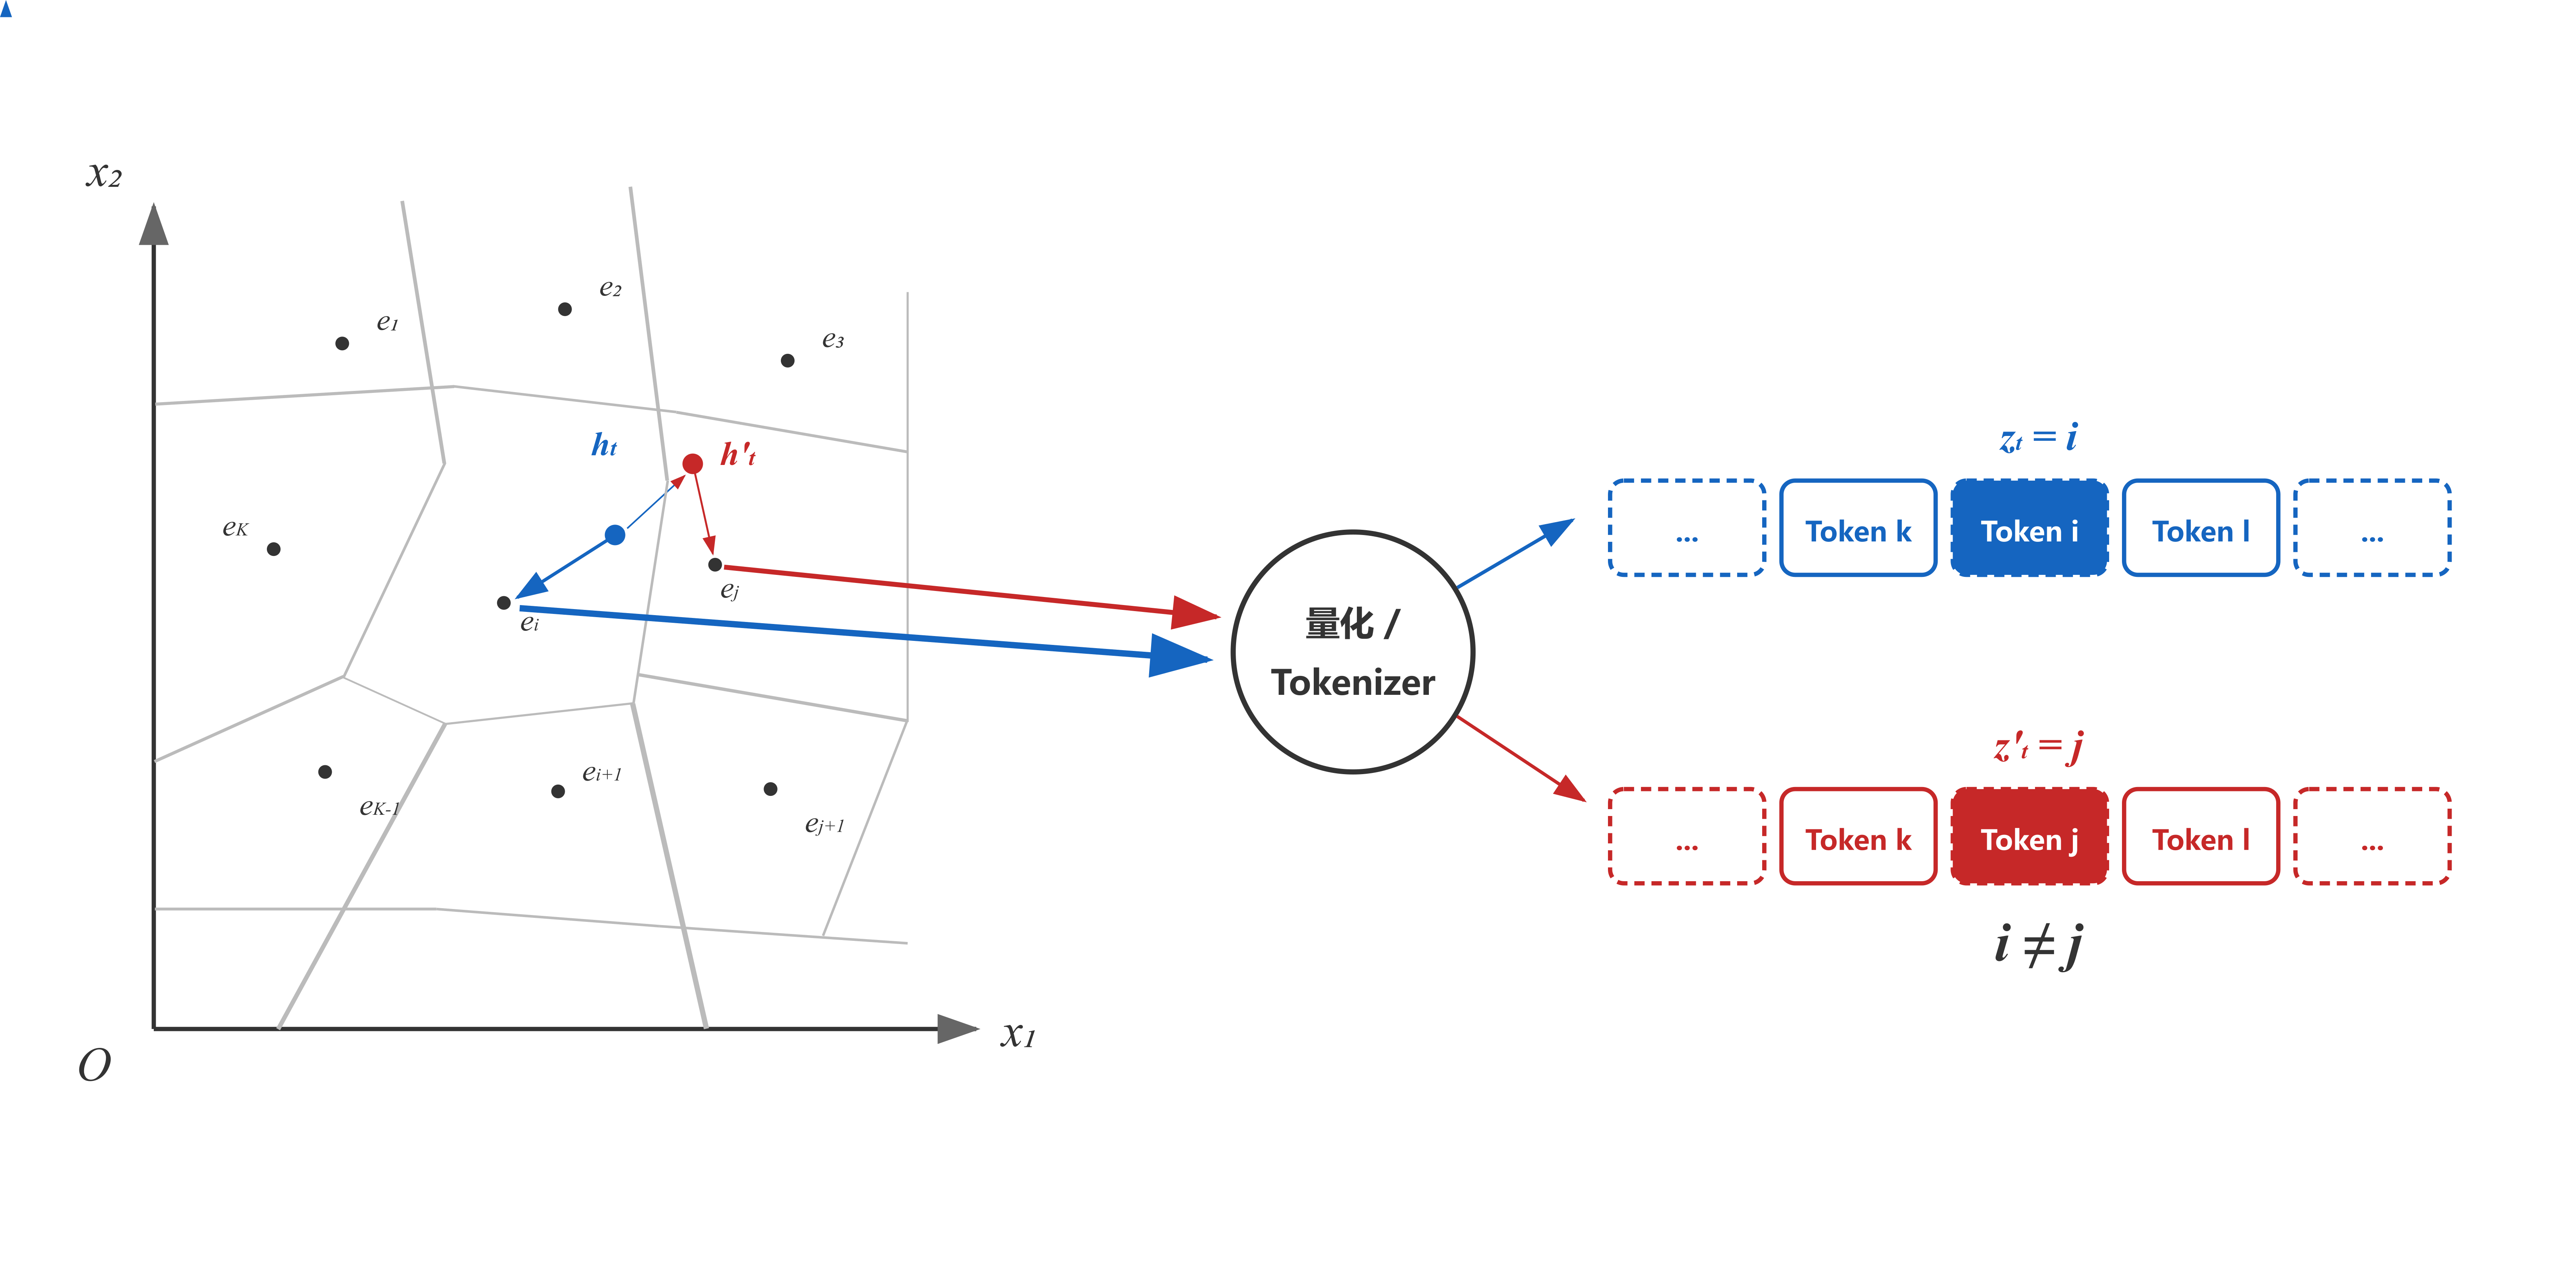
\includegraphics[width=\textwidth,height=0.72\textheight,keepaspectratio]{figures/image6.png}
  \caption{连续表示与离散 token 机制图}
  \label{fig:2-3}
\end{figure}

这种现象不代表大多数语音分词器都会发生大幅 token
跳变，而是使我们将其作为理解离散语音 token
风险的一种机制基础。也就是说，保护扰动首先作用在连续波形和连续表示上；如果目标系统存在语音分词器，连续表示偏移可能进一步传导到离散
token 空间，从而影响后续语言模型或生成模型对参考音频的建模。

\section{说话人识别与声音身份表示}\label{ux8bf4ux8bddux4ebaux8bc6ux522bux4e0eux58f0ux97f3ux8eabux4efdux8868ux793a}

语音克隆系统不仅需要知道参考音频``说了什么''，还需要知道``是谁在说、怎么说''。后者涉及说话人身份、音色、韵律、风格、语速、情绪和声学环境等信息。为了统一描述这些机器可提取的声音条件，本文使用声音身份表示（Voice
Identity Representation）这一上位概念。

\subsection{说话人嵌入与声纹相似度}\label{ux8bf4ux8bddux4ebaux5d4cux5165ux4e0eux58f0ux7eb9ux76f8ux4f3cux5ea6}

说话人嵌入（Speaker
Embedding）是说话人识别和说话人验证中的重要表示形式{[}42-45{]}。它通常将不同长度的语音片段映射为固定维度向量，使系统能够比较两段语音是否来自同一说话人。x-vector
方法使用深度神经网络将可变长度语音映射为固定维度说话人嵌入，并通过数据增强提升鲁棒性\textsuperscript{{[}42{]}}。ECAPA-TDNN（Emphasized
Channel Attention, Propagation and Aggregation in Time Delay Neural
Network）进一步在 TDNN
说话人验证结构中引入通道注意、特征传播和聚合机制，提高说话人表示提取能力\textsuperscript{{[}44{]}}。StyleTTS2
风格编码器和 MFCC 特征也可作为声音条件或声学特征的代理表示{[}46-47{]}。

从语音克隆角度看，说话人嵌入可以作为目标说话人的身份条件。模型一旦能够从公开语音中稳定提取说话人嵌入，就可能在后续生成过程中保持目标说话人的声音身份。因此，主动防护不能只关注自动语音识别结果，也需要关注说话人嵌入和声音身份表示是否仍然稳定对应原始说话人。

声纹相似度（Speaker
Similarity）通常用于衡量两段语音在说话人身份表示空间中的接近程度。常见做法是分别提取两段语音的说话人嵌入，然后计算余弦相似度或其他距离指标。若原始音频与受保护音频在说话人嵌入空间中相似度较高，说明机器仍可能稳定识别其为同一说话人；若相似度下降，则说明保护扰动可能影响了机器对声音身份的提取。

在后续测试与分析中，声纹相似度可作为评价声音身份保护效果的重要指标。需要注意的是，声纹相似度只是声音身份特征链路的一个可观测指标，而不是全部声音身份信息。语音克隆系统还可能依赖音色、韵律、风格、语速和声学环境等条件。因此，本文在术语上使用``声音身份表示''作为上位概念，而不是只用``音色特征''覆盖所有声音条件。

\subsection{声音身份表示}\label{ux58f0ux97f3ux8eabux4efdux8868ux793a}

声音身份表示指机器模型用于表达说话人身份、音色、韵律、风格和声学条件等声音信息的中间表示。它不同于单纯的语义表示。语义表示主要服务于语音内容理解、文本转写和发音结构建模；声音身份表示则主要服务于说话人识别、声音相似度判断和语音合成中的参考声音条件。

在真实语音信号中，语义信息和声音身份信息并不完全解耦。同一句话由不同人说出，会产生不同音色和韵律；同一个说话人在不同情绪、语速、环境下的声音也会发生变化。WavLM
等全栈语音预训练模型的研究背景也表明，语音信号包含说话内容、说话人身份和副语言信息等多方面因素\textsuperscript{{[}39{]}}。因此，V-Guard
在系统设计中采用功能性划分：将``说了什么''归入语义表示链路，将``是谁在说、怎么说''归入声音身份特征链路。这种划分不是声称真实模型内部存在完全独立的两条通道，而是为了明确防护目标和评估口径。

需要说明的是，本文将语音克隆的机器依赖划分为语义表示和声音身份表示两条链路，是从防护目标和评估口径角度提出的功能性划分，并不表示真实语音信号或模型内部存在完全独立的两条通路。语音信号中内容、身份、韵律和声学条件往往相互耦合，采用这一划分是为了更清晰地说明保护扰动分别针对哪些机器处理过程。

\section{对抗攻击与主动防护}\label{ux5bf9ux6297ux653bux51fbux4e0eux4e3bux52a8ux9632ux62a4}

主动防护与对抗样本技术具有一定联系，但二者的安全目标不同。对抗攻击通常以欺骗模型为目标，而
V-Guard
的主动防护目标是保护用户声音资产，降低未授权语音克隆系统对公开语音的利用能力。因此，本节先介绍对抗扰动的基本思想，再说明其如何转化为语音发布前保护机制。

\subsection{对抗攻击与音频对抗样本}\label{ux5bf9ux6297ux653bux51fbux4e0eux97f3ux9891ux5bf9ux6297ux6837ux672c}

对抗样本（Adversarial
Example）指在输入中加入较小扰动，使机器学习模型产生错误输出的样本{[}48-52{]}。投影梯度下降（PGD，Projected
Gradient
Descent）是一类常见的对抗样本优化方法，其核心思想是在扰动幅度受限的约束下，沿着损失函数梯度方向迭代更新输入扰动，并将扰动投影回允许范围内。Madry
等从鲁棒优化角度系统化了 PGD
和一阶对抗者框架\textsuperscript{{[}51{]}}。

对抗样本研究说明，深度神经网络对输入空间中的细粒度变化可能较为敏感。对于图像模型，这种变化可能表现为像素级扰动；对于语音模型，这种变化可能表现为波形或频域中的细粒度信号变化。V-Guard
借鉴的是这种``在受限扰动下影响机器表示''的优化思想，但其目的不是攻击正常服务，而是在用户授权的语音发布前生成保护扰动。

音频对抗样本研究关注如何在语音信号中加入扰动，使自动语音识别系统输出错误文本。与图像相比，音频对抗样本还需要考虑人耳听觉感知、播放设备、环境噪声和空中传播等因素。Qin
等利用听觉掩蔽原理构造更不易被人耳察觉的自动语音识别对抗样本，并讨论了物理环境中的鲁棒性问题\textsuperscript{{[}49-50{]}}。

这些研究为主动语音防护提供了两个启发。第一，语音模型的前端表示和解码结果可能受到细粒度扰动影响。第二，音频扰动不能只考虑机器侧效果，还必须考虑人耳侧可感知性。V-Guard
因此在保护扰动生成中同时考虑语义表示链路、声音身份特征链路和听感约束。

\subsection{主动语音防护}\label{ux4e3bux52a8ux8bedux97f3ux9632ux62a4}

主动语音防护将对抗扰动思想用于声音资产保护。与传统攻击不同，主动防护是在用户授权下对自己的语音进行发布前处理，使公开音频在保持正常可听性的同时降低被未授权克隆的风险。AntiFake
使用对抗音频防止未授权语音合成，其目标是使攻击者基于受保护语音生成的音频不再像目标受害者\textsuperscript{{[}19{]}}。E2E-VGuard
面向生产级 LLM-based 端到端语音合成和 ASR-driven
语音合成流程，进一步讨论了自动转写、编码器集成和心理声学约束在主动防护中的作用\textsuperscript{{[}23{]}}。因此，主动语音防护可以理解为将对抗扰动思想从攻击场景转化为防护场景：扰动不用于规避系统检测，而用于降低未授权模型对用户声音资产的利用价值。相关工作还覆盖语音转换防护、不可学习语音样本、鲁棒语音保护、语音匿名化和黑盒
ASR 隐私保护等方向{[}20-27{]}。

本项目与上述方向一致，属于发布前主动防护范畴。不同的是，本项目更强调系统工程闭环：不仅生成受保护音频，还提供音频上传、预处理、保护模式选择、ASR
转写对比、声纹相似度评估、音频质量评估、可视化展示、历史记录和结果导出等功能。

\section{听觉感知与音频质量评价}\label{ux542cux89c9ux611fux77e5ux4e0eux97f3ux9891ux8d28ux91cfux8bc4ux4ef7}

主动防护必须兼顾防护效果和音频可用性。如果受保护音频明显变吵、失真、刺耳或语义不可辨识，即使机器侧保护效果较强，也难以用于真实内容发布。因此，本作品在设计保护扰动时需要引入听感约束，并在测试阶段从客观指标和主观听感两个角度评价音频质量。

\subsection{听觉掩蔽效应与掩蔽阈值计算}\label{ux542cux89c9ux63a9ux853dux6548ux5e94ux4e0eux63a9ux853dux9608ux503cux8ba1ux7b97}

人耳对不同频率、不同时间位置和不同能量强度的声音敏感度并不相同。强能量语音成分可能掩蔽邻近时间或频率区域中的弱扰动，使部分扰动不容易被听众察觉。这种现象通常称为听觉掩蔽。音频对抗样本研究已经利用心理声学掩蔽原理生成更不易被察觉的扰动\textsuperscript{{[}50,53-54{]}}。

在 V-Guard
中，听觉掩蔽并不是为了隐藏攻击行为，而是为了控制保护扰动对正常收听体验的影响。系统希望保护扰动尽量分布在人耳相对不敏感的位置，同时限制整体扰动幅度，使受保护音频仍保持自然、可懂和可发布。

在针对防范恶意语音克隆等源头防护技术的真实业务场景中，防御机制必须严格遵守``对合法用户隐蔽不可见''的底线。为了在防护效能与听觉保真度之间取得平衡，本系统引入了基于人类听觉系统（HAS）物理与心理特性的心理声学掩蔽阈值计算，以保证对音频的保护具有可用性。全局隐蔽阈值的获取由两部分物理屏蔽效果组合而成：

静态生理屏蔽：人耳自身解剖结构带来的底层感知门槛，即绝对安静听觉阈值（ATH）。

动态声场屏蔽：输入原始音频波形（Wave）中高能量音频成分对周边低能量成分产生的遮蔽效应。

系统将这两部分预算在绝对线性能量域中聚合，得到最终的屏蔽阈值，并以此为红线，严格限制对抗微扰在频域中的能量分布。以下为该阈值提取方法的数学推导与实现细节。

\begin{enumerate}
\def\labelenumi{(\arabic{enumi})}
\item
  隐蔽阈值的两部分来源与特征提取

  为了实现对音频扰动能量的精准捕捉，系统设计了一套基于心理声学掩蔽效应的流水线。其核心架构与数据流向如下图所示：
\end{enumerate}


\begin{figure}[htbp]
  \centering
  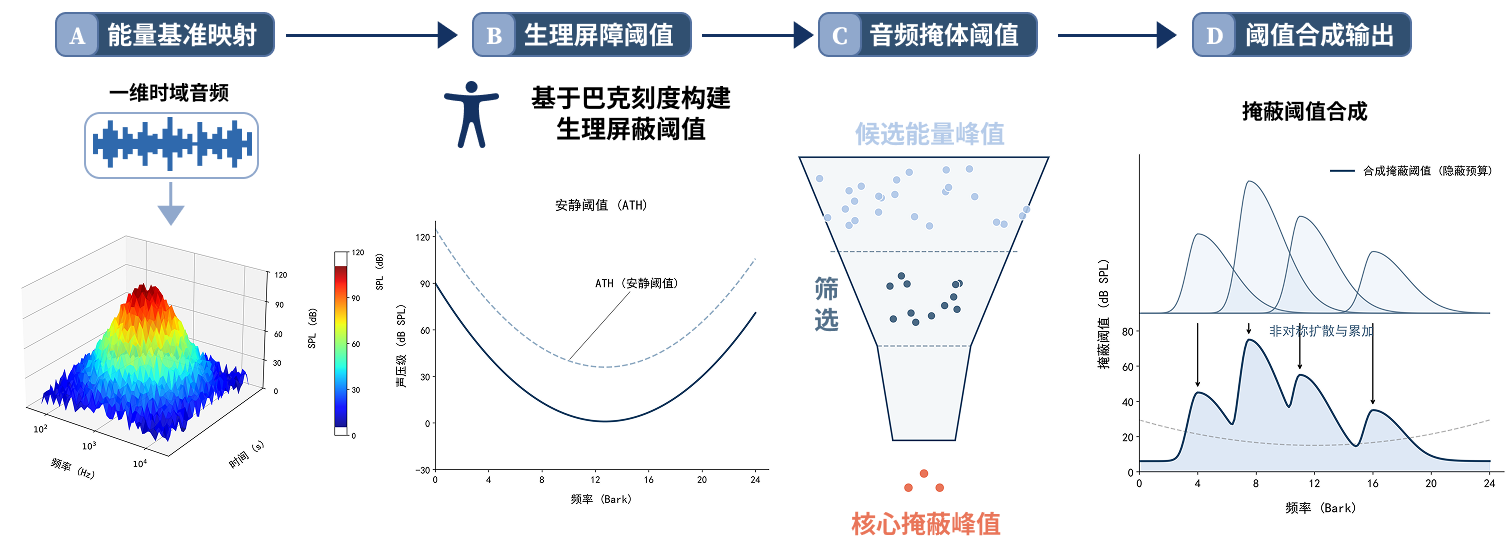
\includegraphics[width=\textwidth,height=0.72\textheight,keepaspectratio]{figures/image7.png}
  \caption{心理声学掩蔽效应的流水线示意图}
  \label{fig:2-4}
\end{figure}

\begin{enumerate}
\def\labelenumi{(\arabic{enumi})}
\setcounter{enumi}{1}
\item
  阈值来源一：人耳静态生理屏蔽（ATH）

  即使在绝对安静的环境中，人耳对不同频率的敏感度也存在非线性的物理底线。系统将线性频率映射至反映耳蜗临界频带特征的巴克刻度（Bark
  Scale, \(z\)），并利用 Terhardt 经验公式计算出绝对听觉阈值曲线：
\end{enumerate}

\[ATH(k) = 3.64 \cdot f_{kHz}(k)^{- 0.8} - 6.5 \cdot e^{- 0.6(f_{kHz}(k) - 3.3)^{2}} + 10^{- 3} \cdot f_{kHz}(k)^{4} - 12\]

其中，\(ATH(k)\)表示第 \(k\) 个频率点处的绝对听觉阈值（单位：dB
SPL），即人耳天然的生理感知下限，\(f_{kHz}(k)\)表示离散频率索引 \(k\)
对应的真实物理频率，单位为千赫兹（kHz）。这条不对称的``浴缸型''曲线构成了隐蔽预算的第一层保底屏障：任何低于此能量限度的扰动，无论声场环境如何，天然不可察觉。

\begin{enumerate}
\def\labelenumi{(\arabic{enumi})}
\setcounter{enumi}{2}
\item
  阈值来源二：输入音频动态屏蔽（同时掩蔽效应）

  当原始语音中存在较高能量的声学刺激（掩蔽音）时，会提升邻近频率的感知门槛。系统在
  \(PSD_{SPL}\)
  中筛选局部极大值作为掩蔽音，并将其及其左右相邻频点的能量在线性域进行聚合。

  每个掩蔽音会向周边频段产生不对称的扩散遮蔽。系统依据频点的 Bark 距离
  \(\Delta z\) 计算扩散裙形包络（Spreading Function,
  \(S_{f}\)）。高频侧的扩散曲线具有强烈的电平依赖性，完美模拟了低频对高频的强烈掩蔽作用：
\end{enumerate}

\[S_{f}(\Delta z) = \left( - 27 + 0.37 \cdot max(E_{masker} - 40,0) \right) \cdot \Delta z\quad(\text{当}\Delta z \geq 0)\]

其中，\(S_{f}(\Delta z)\)表示掩蔽音向高频侧的不对称扩散衰减量（单位：dB），\(\Delta z\)表示目标考察频率与掩蔽音中心频率在巴克（Bark）尺度上的距离，\(E_{masker}\)表示当前掩蔽音聚合了相邻频段能量后的实际总声压级能量（单位：dB
SPL）。

综上，结合局部最大值的聚合能量\(E_{masker}\)、根据\(S_{f}\)计算得到的扩散形状衰减以及依照频率设置的掩蔽偏移常量
\(\Delta_{m}\)，得到了当前单一掩蔽音对全部物理频段所建立的屏蔽山峰矩阵分布线
\(T_m(k)\)：

\[T_m(k)=E_{masker}+\Delta_m+S_f(\Delta z(k))\]

\begin{enumerate}
\def\labelenumi{(\arabic{enumi})}
\setcounter{enumi}{3}
\item
  屏蔽预算组合：全局阈值合成

  为了获得最终的全局屏蔽阈值
  \(\Theta(x)\)，系统必须将``人耳静态屏蔽（ATH）''与所有的``动态声场屏蔽（\(T_{m}\)）''脱离对数
  dB 单位，反解回最底层的绝对线性能量功率域进行物理叠加：
\end{enumerate}

\[T_{frame}(k) = 10^{\frac{ATH(k)}{10}} + \sum_{m = 1}^{M}10^{\frac{T_{m}(k)}{10}}\]

在外层包裹着对所有时间帧的时序流转迭代后，所有时域切片的阈值数据被封箱打包，输出为最终的二维矩阵对象\(\Theta(x)\)。至此，一条普通的数字化声压波形，被彻底解构为人类听觉察觉上限的隐蔽预算热力图谱。

\subsection{扰动约束与音频质量评价指标}\label{ux6270ux52a8ux7ea6ux675fux4e0eux97f3ux9891ux8d28ux91cfux8bc4ux4ef7ux6307ux6807}

扰动幅度约束用于限制保护音频与原始音频之间的整体数值差异。仅依靠心理声学约束并不足够，因为某些扰动即使局部不明显，也可能在整体上造成能量偏移或音质下降。相反，仅控制扰动幅度也不能保证扰动分布在人耳不敏感区域。因此，主动防护通常需要同时考虑扰动幅度约束和听感约束。

在后续系统核心技术中，保护扰动会作为待优化变量进行迭代更新。每轮更新后，系统需要控制扰动不超过设定范围，并将受保护音频裁剪到合法波形区间。这样可以避免保护扰动无限增大，保证系统输出仍然是可正常播放的音频文件。

音频质量评价可以从多个角度进行。信噪比（SNR，Signal-to-Noise
Ratio）用于衡量信号能量与噪声或扰动能量之间的比例，能够反映受保护音频与原始音频之间的整体差异。感知语音质量评估（PESQ，Perceptual
Evaluation of Speech
Quality）是一种用于端到端语音质量客观评价的方法，曾作为 ITU-T P.862
标准的一部分用于窄带电话网络和语音编解码器质量评估\textsuperscript{{[}55{]}}。短时客观可懂度（STOI，Short-Time
Objective
Intelligibility）用于预测噪声或时频加权语音的可懂度，适合辅助评价语音内容是否仍可被正常理解\textsuperscript{{[}56{]}}。主观平均意见分（MOS）评价通常可参照
ITU-T P.800 的主观听评方法{[}57{]}。

除客观指标外，波形图、频谱图和主观试听也很重要。波形图可以展示保护前后整体振幅变化，频谱图可以展示扰动在时间---频率空间中的分布，主观试听则直接反映用户是否能够接受受保护音频。V-Guard
后续测试章节将结合 ASR
转写、声音身份相似度、SNR、PESQ、STOI、波形图、频谱图和主观听感，对保护效果与音频可用性进行综合分析。

综上，本章从语音合成、语音表示、声音身份表示、主动防护和音频质量评价五个方面介绍了
V-Guard
的技术背景。可以看到，现代语音克隆系统依赖的不只是最终文本输出，而是包括语义表示、声音身份表示、连续语音表示和离散语音
token 在内的多层机器表示。V-Guard
的系统设计正是建立在这一认识之上：通过发布前保护扰动影响机器对公开语音的稳定提取，同时利用听感约束保证受保护音频仍具有正常使用价值。

\FloatBarrier
